

%% NJCTL: PSI AP Physics C
%%----------------------------------------


%% Work and Energy with Calculus
%%----------------------------------------
\element{njctl}{
\begin{question}{work-calculus-q01}
    An object moves according to the function $x=t^{7/2}$ where $x$ is the distance traveled and $t$ is the time.
    Its kinetic energy is proportional to:
    \begin{multicols}{3}
    \begin{choices}
        \wrongchoice{$t^{5/2}$}
        \wrongchoice{$t^{7/2}$}
      \correctchoice{$t^{5}$}
        \wrongchoice{$t^{3/2}$}
        \wrongchoice{$t^{7}$}
    \end{choices}
    \end{multicols}
\end{question}
}

\element{njctl}{
\begin{question}{work-calculus-q02}
    Which of the following best describes the relationship between force and potential energy?
    \begin{choices}
        \wrongchoice{Force is the anti-derivative of potential energy.}
      \correctchoice{Force is the negative gradient of potential energy.}
        \wrongchoice{Potential energy is the negative gradient of force.}
        \wrongchoice{Potential energy is the derivative of force.}
        \wrongchoice{Force is the anti-derivative of potential energy.}
    \end{choices}
\end{question}
}

\element{njctl}{
\begin{question}{work-calculus-q03}
    A \SI{5}{\kilo\gram} ball moves in the $x$ direction where $x$ represents the ball's position.
    The potential energy $U$ of the ball in Joules is given as a function:
    \begin{equation*}
        U(x) = 4x^2 - 3x + 2\,.
    \end{equation*}
    The force on the particle at $x=\SI{4}{\meter}$ is:
    \begin{choices}
      \correctchoice{\SI{29}{\newton} in the $-x$ direction}
        \wrongchoice{\SI{29}{\newton} in the $+x$ direction}
        \wrongchoice{\SI{108}{\newton} in the $-x$ direction}
        \wrongchoice{\SI{45}{\newton} in the $-x$ direction}
        \wrongchoice{\SI{108}{\newton} in the $+x$ direction}
    \end{choices}
\end{question}
}

\element{njctl}{
\begin{question}{work-calculus-q04}
    A student pushes a box across a rough, flat surface at a constant speed $v$.
    The box has a mass $m$,
        and the coefficient of sliding friction is represented by $\mu$.
    The power supplied by the person to the box is:
    \begin{multicols}{3}
    \begin{choices}
        \wrongchoice{zero}
        \wrongchoice{$\dfrac{\mu mg}{v}$}
        \wrongchoice{$\dfrac{\mu v}{mg}$}
        \wrongchoice{$\dfrac{mg}{\mu v}$}
      \correctchoice{$\mu mgv$}
    \end{choices}
    \end{multicols}
\end{question}
}

\element{njctl}{
\begin{question}{work-calculus-q05}
    The force exerted by a spring is given by:
    \begin{equation*}
        F = \dfrac{kx^4}{2}\, .
    \end{equation*}
    %% corrected  mistake
    If $k$ is \SI{100}{\newton\per\meter\tothefourth},
        find the work done by the spring on a mass from $x=\SI{0}{\meter}$ to $x=\SI{2}{\meter}$.
    \begin{multicols}{3}
    \begin{choices}
        \wrongchoice{\SI{100}{\joule}}
      \correctchoice{\SI{320}{\joule}}
        \wrongchoice{\SI{800}{\joule}}
        \wrongchoice{\SI{1600}{\joule}}
        \wrongchoice{\SI{2400}{\joule}}
    \end{choices}
    \end{multicols}
\end{question}
}

\element{njctl}{
\begin{question}{work-calculus-q06}
    A man lifts a mass $m$ at constant speed to a height $h$ in time $t$.
    How much work is done by the weight lifter on the mass?
    \begin{multicols}{3}
    \begin{choices}
        \wrongchoice{$mgt$}
        \wrongchoice{zero}
      \correctchoice{$mgh$}
        \wrongchoice{$\dfrac{mgh}{t}$}
        \wrongchoice{$\dfrac{mgt}{h}$}
    \end{choices}
    \end{multicols}
\end{question}
}

\element{njctl}{
\begin{question}{work-calculus-q07}
    A spring force is given by the formula $F=20x-12x^2$,
        where $F$ is in newtons and $x$ is in meters.
    What is the change in potential energy when the spring is stretched \SI{3}{\meter} from its equilibrium position?
    \begin{multicols}{3}
    \begin{choices}
      \correctchoice{\SI{18}{\joule}}
        \wrongchoice{\SI{-18}{\joule}}
        \wrongchoice{\SI{56}{\joule}}
        \wrongchoice{\SI{-56}{\joule}}
        \wrongchoice{\SI{64}{\joule}}
    \end{choices}
    \end{multicols}
\end{question}
}

%\element{njctl}{
%\begin{question}{work-calculus-q08}
%    On top of a skyscraper of height $H$,
%        a ball of mass $m$ is thrown directly downward with an initial speed $v_0$.
%    What is the speed of the ball before it strikes the ground?
%    Ignore air resistance.
%    \begin{multicols}{2}
%    \begin{choices}
%        %% NOTE: v_f does not make sense, that is the asked for quantity
%        \wrongchoice{$mgh - \dfrac{1}{2}m\left(v_0^2-v_f^2\right)$}
%        \wrongchoice{$mgh - \dfrac{1}{2}m\left(v_0^2+v_f^2\right)$}
%        \wrongchoice{$mgh - \dfrac{1}{2}m\left(v_f^2-v_0^2\right)$}
%      \correctchoice{$\sqrt{v_0^2 + 2gh}$}
%        \wrongchoice{$\dfrac{1}{2}m\left(v_f^2-v_0^2\right) - mgh$}
%    \end{choices}
%    \end{multicols}
%\end{question}
%}
%
%\element{njctl}{
%\begin{question}{work-calculus-q09}
%    A ball attached to a string rotates in a complete circle at a constant speed.
%    The work done during each revolution is:
%    \begin{multicols}{3}
%    \begin{choices}
%        %% NOTE: define symbols?
%      \correctchoice{zero}
%        \wrongchoice{$U$}
%        \wrongchoice{$U+Ke$}
%        \wrongchoice{$Ke$}
%        \wrongchoice{$Ke-U$}
%    \end{choices}
%    \end{multicols}
%\end{question}
%}

\element{njctl}{
\begin{question}{work-calculus-q10}
    The potential energy of two molecules is given by: $U=\dfrac{2}{r^7}-\dfrac{4}{r^5}$.
    If $r$ is the distance between two molecules,
        what is the force acting on the particles if $r=\SI{1}{\meter}$?
    \begin{multicols}{3}
    \begin{choices}
        \wrongchoice{\SI{0.75}{\newton}}
        \wrongchoice{\SI{0.67}{\newton}}
        \wrongchoice{\SI{2}{\newton}}
      \correctchoice{\SI{-6}{\newton}}
        \wrongchoice{\SI{10}{\newton}}
    \end{choices}
    \end{multicols}
\end{question}
}

\element{njctl}{
\begin{question}{work-calculus-q11}
    A force of \SI{40}{\newton} compresses a spring with a spring constant \SI{80}{\newton\per\meter}.
    How much energy is stored in the spring?
    \begin{multicols}{3}
    \begin{choices}
      \correctchoice{\SI{10}{\joule}}
        \wrongchoice{\SI{15}{\joule}}
        \wrongchoice{\SI{20}{\joule}}
        \wrongchoice{\SI{25}{\joule}}
        \wrongchoice{\SI{30}{\joule}}
    \end{choices}
    \end{multicols}
\end{question}
}

\element{njctl}{
\begin{question}{work-calculus-q12}
    What is the power delivered by gravity to a \SI{6}{\kilo\gram} block \SI{4}{\second} after it has fallen from rest?
    \begin{multicols}{3}
    \begin{choices}
        \wrongchoice{\SI{2400}{\watt}}
        \wrongchoice{\SI{1000}{\watt}}
        \wrongchoice{\SI{800}{\watt}}
      \correctchoice{\SI{1200}{\watt}}
        \wrongchoice{\SI{2000}{\watt}}
    \end{choices}
    \end{multicols}
\end{question}
}

\element{njctl}{
\begin{question}{work-calculus-q13}
    If $F(x) = 8x^3 -3x^2$,
        where $F$ is in newtons and $x$ is in meters,
        what is the work done from $x=\SI{1}{\meter}$ to $x=\SI{2}{\meter}$?
    \begin{multicols}{3}
    \begin{choices}
        \wrongchoice{\SI{0.5}{\joule}}
        \wrongchoice{\SI{0.8}{\joule}}
        \wrongchoice{\SI{2}{\joule}}
        \wrongchoice{\SI{12}{\joule}}
      \correctchoice{\SI{23}{\joule}}
    \end{choices}
    \end{multicols}
\end{question}
}

\element{njctl}{
\begin{question}{work-calculus-q14}
    A \SI{2}{\kilo\gram} block is pushed horizontally across a rough surface with a coefficient of kinetic friction of \num{0.2},
        at a constant speed of \SI{4}{\meter\per\second}, by a force $F$.
    The work that is done by the force in \SI{5}{\second} is:
    \begin{multicols}{3}
    \begin{choices}
        \wrongchoice{\SI{20}{\joule}}
        \wrongchoice{\SI{40}{\joule}}
        \wrongchoice{\SI{60}{\joule}}
      \correctchoice{\SI{80}{\joule}}
        \wrongchoice{\SI{100}{\joule}}
    \end{choices}
    \end{multicols}
\end{question}
}

\element{njctl}{
\begin{question}{work-calculus-q15}
    A constant force supplies an average power of \SI{8}{\watt} to a box during a certain time interval.
    If the box has an average speed of \SI{4}{\meter\per\second},
        and the force acts in the same direction as motion of the object,
        the magnitude of the force is:
    \begin{multicols}{3}
    \begin{choices}
        \wrongchoice{\SI{1}{\newton}}
      \correctchoice{\SI{2}{\newton}}
        \wrongchoice{\SI{4}{\newton}}
        \wrongchoice{\SI{6}{\newton}}
        \wrongchoice{\SI{8}{\newton}}
    \end{choices}
    \end{multicols}
\end{question}
}

\element{njctl}{
\begin{question}{work-calculus-q16}
    Which of the following is true about an oscillating system in simple harmonic motion?
    \begin{choices}
        \wrongchoice{Potential energy is never equal to kinetic energy.}
        \wrongchoice{Potential energy is equal to kinetic energy at all points.}
        \wrongchoice{Potential energy decreases all the time.}
        \wrongchoice{Kinetic energy increases all the time.}
      \correctchoice{Maximum potential energy is equal to maximum kinetic energy.}
    \end{choices}
\end{question}
}

\element{njctl}{
\begin{question}{work-calculus-q17}
    A \SI{4}{\kilo\gram} mass is moving with a velocity given by $v(t)=\dfrac{1}{4}t^4$.
    At $t=\SI{1}{\second}$,
        the instantaneous power delivered by the net force is:
    \begin{multicols}{3}
    \begin{choices}
      \correctchoice{\SI{1}{\watt}}
        \wrongchoice{\SI{3}{\watt}}
        \wrongchoice{\SI{12}{\watt}}
        \wrongchoice{\SI{14}{\watt}}
        \wrongchoice{\SI{20}{\watt}}
    \end{choices}
    \end{multicols}
\end{question}
}

\element{njctl}{
\begin{question}{work-calculus-q18}
    What is the instantaneous power delivered by the net force at $t=\SI{2}{\second}$ to a \SI{2}{\kilo\gram} mass moving according to $x(t)=\dfrac{1}{3} t^3$?
    \begin{multicols}{3}
    \begin{choices}
        \wrongchoice{\SI{2}{\watt}}
        \wrongchoice{\SI{10}{\watt}}
        \wrongchoice{\SI{16}{\watt}}
        \wrongchoice{\SI{24}{\watt}}
      \correctchoice{\SI{32}{\watt}}
    \end{choices}
    \end{multicols}
\end{question}
}

\element{njctl}{
\begin{question}{work-calculus-q19}
    A particle of mass $m$ follows the potential energy graph as shown below.
    \begin{center}
    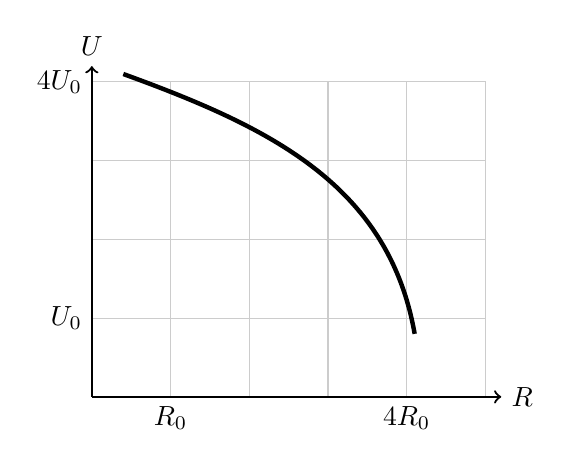
\begin{tikzpicture}
        %% Axis
        \draw[step=1cm,thin,white!80!black] (0,0) grid (5,4);
        \draw[thick,->] (0,0) -- (0,4.2) node[anchor=south] {$U$};
        \draw[thick,->] (0,0) -- (5.2,0) node[anchor=west] {$R$};
        \node[anchor=east] at (0,1) {$U_0$};
        \node[anchor=east] at (0,4) {$4U_0$};
        \node[anchor=north] at (1,0) {$R_0$};
        \node[anchor=north] at (4,0) {$4R_0$};
        %% function
        \draw[ultra thick] (0.4,4.1) to[out=340,in=100,tension=1.0] (4.1,0.8);
    \end{tikzpicture}
    \end{center}
    The particle is initially at rest at $R_0$.
    Determine the particle's speed at position $4R_0$.
    \begin{multicols}{3}
    \begin{choices}
        \wrongchoice{$\sqrt{\dfrac{U_0}{m}}$}
        \wrongchoice{$\sqrt{\dfrac{2 U_0}{m}}$}
        \wrongchoice{$\sqrt{\dfrac{4 U_0}{m}}$}
      \correctchoice{$\sqrt{\dfrac{6 U_0}{m}}$}
        \wrongchoice{$\sqrt{\dfrac{8 U_0}{m}}$}
    \end{choices}
    \end{multicols}
\end{question}
}

\element{njctl}{
\begin{question}{work-calculus-q20}
    The function $U(r) = ar^{-3/2} + b$ represents the potential energy of a particle,
        where $a$ and $b$ are positive constants,
        which of the following is an expression for the force on the particle?
    \begin{multicols}{3}
    \begin{choices}
      \correctchoice{$\dfrac{3}{2} ar^{-5/2}$}
        \wrongchoice{$2 ar^{-1/2}$}
        \wrongchoice{$-\dfrac{3}{2} ar^{-5/2}$}
        \wrongchoice{$-\dfrac{1}{2} ar^{-5/2}$}
        \wrongchoice{$\dfrac{1}{2} ar^{-3/2}$}
    \end{choices}
    \end{multicols}
\end{question}
}

\element{njctl}{
\begin{question}{work-calculus-q21}
    A mass moves under the influence of a potential energy given by:
    \begin{equation*}
        U(x) = x^3 - 2x^2\,.
    \end{equation*}
    At $x=\SI{2}{\meter}$,
        the force on the mass will be:
    \begin{multicols}{2}
    \begin{choices}
        \wrongchoice{\SI{4}{\newton}, $+$ direction}
      \correctchoice{\SI{4}{\newton}, $-$ direction}
        \wrongchoice{\SI{3}{\newton}, $+$ direction}
        \wrongchoice{\SI{3}{\newton}, $-$ direction}
        \wrongchoice{\SI{7}{\newton}, $+$ direction}
    \end{choices}
    \end{multicols}
\end{question}
}

\element{njctl}{
\begin{question}{work-calculus-q22}
    A \SI{6}{\kilo\gram} object's potential energy is represented by:
    \begin{equation*}
        U(r) = 9r^2 + 4 \,,
    \end{equation*}
    where all quantities are in base SI units.
    Find the acceleration of the object at $r=\SI{2}{\meter}$.
    \begin{multicols}{3}
    \begin{choices}
        \wrongchoice{\SI{-4}{\meter\per\second\squared}}
        \wrongchoice{\SI{4}{\meter\per\second\squared}}
      \correctchoice{\SI{-6}{\meter\per\second\squared}}
        \wrongchoice{\SI{6}{\meter\per\second\squared}}
        \wrongchoice{\SI{12}{\meter\per\second\squared}}
    \end{choices}
    \end{multicols}
\end{question}
}

\element{njctl}{
\begin{question}{work-calculus-q23}
    A restoring force $F=-2x^3$ acts on an object,
        where $x$ is the displacement of the object from its equilibrium position.
    How much work must be done by an external force to move the object from $x=0$ to $x=\SI{2}{\meter}$?
    \begin{multicols}{3}
    \begin{choices}
        \wrongchoice{\SI{2}{\joule}}
        \wrongchoice{\SI{24}{\joule}}
      \correctchoice{\SI{8}{\joule}}
        \wrongchoice{\SI{10}{\joule}}
        \wrongchoice{\SI{15}{\joule}}
    \end{choices}
    \end{multicols}
\end{question}
}

\element{njctl}{
\begin{question}{work-calculus-q24}
    How much work is done by an external force in stretching a spring from $x=0$ to $x=\SI{0.2}{\meter}$,
        whose restoring force varies according to the following formula:
        $F(x) = -\left(\SI{6}{\newton\per\meter}\right) x + \left(\SI{30}{\newton\per\meter\squared}\right) x^2$?
    \begin{multicols}{3}
    \begin{choices}
        \wrongchoice{\SI{-0.04}{\joule}}
      \correctchoice{\SI{0.04}{\joule}}
        \wrongchoice{\SI{-0.16}{\joule}}
        \wrongchoice{\SI{0.16}{\joule}}
        \wrongchoice{\SI{0.08}{\joule}}
    \end{choices}
    \end{multicols}
\end{question}
}

\element{njctl}{
\begin{question}{work-calculus-q25}
    The restoring force of a spring varies with displacement according to:
        $F = -kx^2$.
    What is the potential energy of the spring when it is stretched by a distance $D$ from equilibrium?
    \begin{multicols}{3}
    \begin{choices}
        \wrongchoice{$\dfrac{kD^2}{3}$}
        \wrongchoice{$\dfrac{kD^2}{4}$}
      \correctchoice{$\dfrac{kD^3}{3}$}
        \wrongchoice{$\dfrac{kD^2}{2}$}
        \wrongchoice{$\dfrac{kD^3}{2}$}
    \end{choices}
    \end{multicols}
\end{question}
}

\element{njctl}{
\begin{question}{work-calculus-q26}
    The potential energy of a spring is given by the following formula:
    \begin{equation*}
        U(x) = \dfrac{1}{3}\alpha x^3 - \beta x\, ,
    \end{equation*}
    where $\alpha$ and $\beta$ are positive constants.
    Which of the following represents the restoring force of the spring?
    \begin{multicols}{2}
    \begin{choices}
        \wrongchoice{$3\alpha x^2 - \beta$}
        \wrongchoice{$-3\alpha x^2 + \beta$}
        \wrongchoice{$2\alpha x^3 - \beta x$}
        \wrongchoice{$3\alpha x - \beta$}
      \correctchoice{$-\alpha x^2 + \beta$}
    \end{choices}
    \end{multicols}
\end{question}
}

\element{njctl}{
\begin{question}{work-calculus-q27}
    The potential energy of a spring is given by the following formula:
    \begin{equation*}
        U(x) = \dfrac{1}{3}\alpha x^3 - \dfrac{1}{2}\beta x^2\, ,
    \end{equation*}
    where $\alpha$ and $\beta$ are positive constants.
    What is the location(s) of the equilibrium points?
    \begin{choices}
        \wrongchoice{$x=0$ only}
        \wrongchoice{$x=\dfrac{\beta}{\alpha}$ only}
      \correctchoice{$x=0$ and $x=\dfrac{\beta}{\alpha}$ only}
        \wrongchoice{$x=0$ and $x=\dfrac{2\beta}{\alpha}$ only }
        \wrongchoice{$x=\dfrac{3\beta}{2\alpha}$ only}
    \end{choices}
\end{question}
}

\element{njctl}{
\begin{question}{work-calculus-q28}
    The gravitational force between a spaceship and Earth is given by the formula:
    \begin{equation*}
        F = - \dfrac{GMm}{r^2}\, .
    \end{equation*}
    Which of the following represents the potential energy of the spaceship/Earth system,
        assuming that $U=0$ when $r\to\infty$.
    \begin{multicols}{2}
    \begin{choices}
        \wrongchoice{$U = \dfrac{GMm}{r^3}$}
        \wrongchoice{$U = \dfrac{GMm}{r^2}$}
        \wrongchoice{$U = \dfrac{GM}{r}$}
        \wrongchoice{$U = \dfrac{GMm}{r}$}
      \correctchoice{$U = -\dfrac{GMm}{r}$}
    \end{choices}
    \end{multicols}
\end{question}
}

\element{njctl}{
\begin{question}{work-calculus-q29}
    A conservative force parallel to the $x$-axis moves a particle along the $x$-axis.
    The potential energy of the particle is given by
    \begin{equation*}
        U(x) = \dfrac{1}{4}\alpha x^4\, ,
    \end{equation*}
    where $\alpha=\SI{0.5}{\joule\per\meter\tothefourth}$.
    What is the force on the particle when it is located at $x=\SI{2}{\meter}$?
    \begin{multicols}{3}
    \begin{choices}
      \correctchoice{\SI{-4}{\newton}}
        \wrongchoice{\SI{4}{\newton}}
        \wrongchoice{\SI{8}{\newton}}
        \wrongchoice{\SI{-8}{\newton}}
        \wrongchoice{\SI{10}{\newton}}
    \end{choices}
    \end{multicols}
\end{question}
}

\element{njctl}{
\begin{question}{work-calculus-q30}
    A conservative force parallel to the $x$-axis moves a particle along the $x$-axis.
    The potential energy of the particle is given by
    \begin{equation*}
        U(x) = -\dfrac{\alpha}{x^2} \, ,
    \end{equation*}
    where $\alpha$ is a positive constant.
    Which of the following represents the force on the particle?
    \begin{multicols}{3}
    \begin{choices}
        \wrongchoice{$\dfrac{2\alpha}{x}$}
        \wrongchoice{$-\dfrac{2\alpha}{x}$}
        \wrongchoice{$\dfrac{3\alpha}{x}$}
        \wrongchoice{$\dfrac{2\alpha}{x^2}$}
      \correctchoice{$-\dfrac{2\alpha}{x^3}$}
    \end{choices}
    \end{multicols}
\end{question}
}

\newcommand{\PSIapcWorkCalculusQThirtyOne}{
\begin{tikzpicture}
    \begin{axis}[
        axis y line=left,
        axis x line=bottom,
        axis line style={->},
        xlabel={time},
        x unit=\si{\second},
        xtick={0,2,4,6},
        minor x tick num=1,
        ylabel={force},
        y unit=\si{\newton},
        ytick={0,2,4,6},
        minor y tick num=1,
        xmin=0,xmax=6.5,
        ymin=0,ymax=6.5,
        width=0.8\columnwidth,
        height=0.5\columnwidth,
        grid=both,
        very thin,
    ]
    %% TODO: draw graph function
    %% NOTE: smooth plot through coordinates
    %% NOTE: then add circle and letter label after
    \addplot[line width=1pt,mark=\empty] plot coordinates {(0,6) (4,6) (6,0) };
    \end{axis}
\end{tikzpicture}
}

%\element{njctl}{
%\begin{question}{work-calculus-q31}
%    A conservative force parallel to the $x$-axis moves a particle along the $x$-axis.
%    The potential energy as a function of position is presented by the graph.
%    \begin{center}
%        \PSIapcWorkCalculusQThirtyOne
%    \end{center}
%    The particle is released from rest at point $A$.
%    What is the approximate force on the particle when it passes point $B$?
%    \begin{multicols}{3}
%    \begin{choices}
%      \correctchoice{\SI{3}{\newton}}
%        \wrongchoice{\SI{1}{\newton}}
%        \wrongchoice{\SI{-3}{\newton}}
%        \wrongchoice{\SI{6}{\newton}}
%        \wrongchoice{\SI{-6}{\newton}}
%    \end{choices}
%    \end{multicols}
%\end{question}
%}

%\element{njctl}{
%\begin{question}{work-calculus-q32}
%    A conservative force parallel to the $x$-axis moves a particle along the $x$-axis.
%    The potential energy as a function of position is presented by the graph.
%    \begin{center}
%        \PSIapcWorkCalculusQThirtyOne
%    \end{center}
%    The particle is released from rest at point $A$.
%    At what location(s) is the particle in a stable equilibrium?
%    \begin{choices}
%        \wrongchoice{$x=\SI{1.0}{\meter}$ only}
%        \wrongchoice{$x=\SI{2.0}{\meter}$ only}
%        \wrongchoice{$x=\SI{4.0}{\meter}$ only}
%        \wrongchoice{$x=\SI{2.0}{\meter}$ and $x=\SI{4}{\meter}$ only}
%      \correctchoice{$x=\SI{2.0}{\meter}$ and $x=\SI{5.6}{\meter}$ only}
%    \end{choices}
%\end{question}
%}

%\element{njctl}{
%\begin{question}{work-calculus-q33}
%    A conservative force parallel to the $x$-axis moves a particle along the $x$-axis.
%    The potential energy as a function of position is presented by the graph.
%    \begin{center}
%        \PSIapcWorkCalculusQThirtyOne
%    \end{center}
%    The particle is released from rest at point $A$.
%    What is the largest value of $x$ reached by the particle during this motion?
%    \begin{multicols}{3}
%    \begin{choices}
%        \wrongchoice{\SI{5.6}{\meter}}
%        \wrongchoice{\SI{4.0}{\meter}}
%      \correctchoice{\SI{6.9}{\meter}}
%        \wrongchoice{\SI{8.0}{\meter}}
%        \wrongchoice{\SI{2.0}{\meter}}
%    \end{choices}
%    \end{multicols}
%\end{question}
%}

%\element{njctl}{
%\begin{question}{work-calculus-q34}
%    A conservative force parallel to the $x$-axis moves a particle along the $x$-axis.
%    The potential energy as a function of position is presented by the graph.
%    \begin{center}
%        \PSIapcWorkCalculusQThirtyOne
%    \end{center}
%    The particle is released from rest at point $A$.
%    At what location(s) is the particle is in unstable equilibrium?
%    \begin{choices}
%        \wrongchoice{$x=\SI{1.0}{\meter}$ only}
%        \wrongchoice{$x=\SI{2.0}{\meter}$ only}
%      \correctchoice{$x=\SI{4.0}{\meter}$ only}
%        \wrongchoice{$x=\SI{2.0}{\meter}$ and $x=\SI{4}{\meter}$ only}
%        \wrongchoice{$x=\SI{2.0}{\meter}$ and $x=\SI{5.6}{\meter}$ only}
%    \end{choices}
%\end{question}
%}

%\element{njctl}{
%\begin{question}{work-calculus-q35}
%    A conservative force parallel to the $x$-axis moves a particle along the $x$-axis.
%    The potential energy as a function of position is presented by the graph.
%    \begin{center}
%        \PSIapcWorkCalculusQThirtyOne
%    \end{center}
%    The particle is released from rest at point $A$.
%    What is the approximate force on the particle when it passes point $D$?
%    \begin{multicols}{3}
%    \begin{choices}
%        \wrongchoice{\SI{2}{\newton}}
%      \correctchoice{\SI{-2}{\newton}}
%        \wrongchoice{\SI{-3}{\newton}}
%        \wrongchoice{\SI{-4}{\newton}}
%        \wrongchoice{\SI{-6}{\newton}}
%    \end{choices}
%    \end{multicols}
%\end{question}
%}


\endinput


